\subsubsection*{One Particle simulation}\label{sec:OnePart}

We conducted a simulation of a single particle using both the FE and the RK4 method to evolve the Penning trap over a total time frame of $50 \mu s$. 
For the setup of the trap, we used the conditions outlined in \cref{sec:penningtrap}, while initialising the particle at the position $\bold{r}=(20, 0, 20) \mu m$ with the velocity $\bold{v} = (0, 25, 0)\mu m/\mu s$.
\begin{figure}[h]
    \centering
    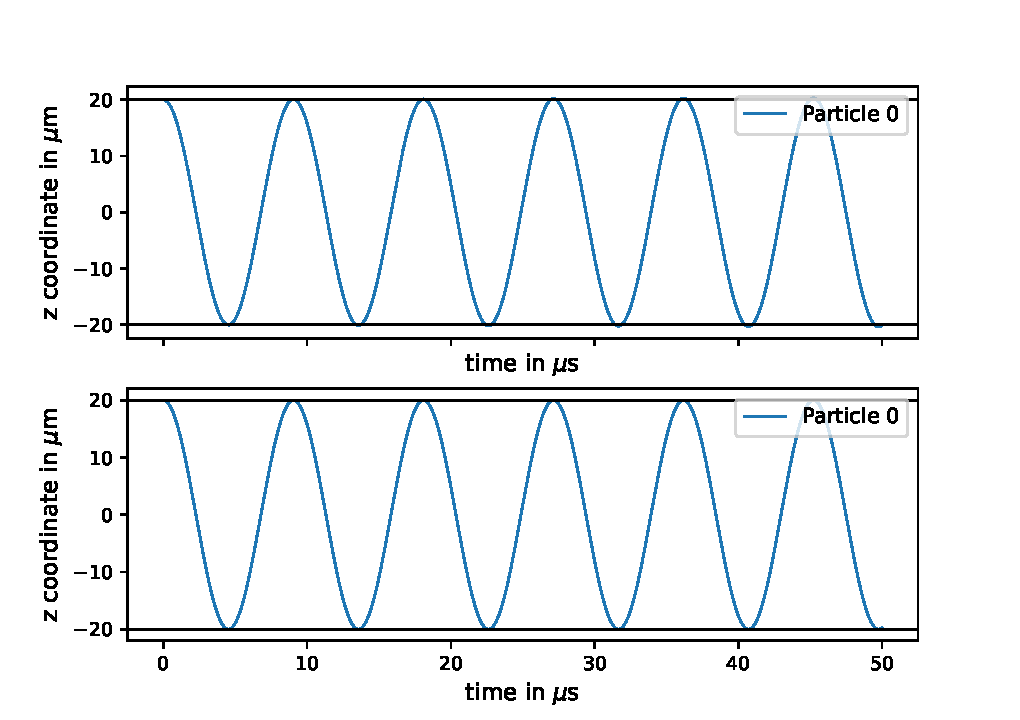
\includegraphics[width = 0.45 \textwidth]{Figures/RK4_vs_FE_z-t-plot.pdf}
    \caption{Evolution of the z-coordinate of a single particle over 50 $\mu s$. The upper plot shows the simulation using FE with 32000 time steps, the lower plot shows the simulation using RK4 with 32000 time steps.}
    \label{fig:z-t-singleparticle}
\end{figure}

\begin{figure}[h]
    \centering
    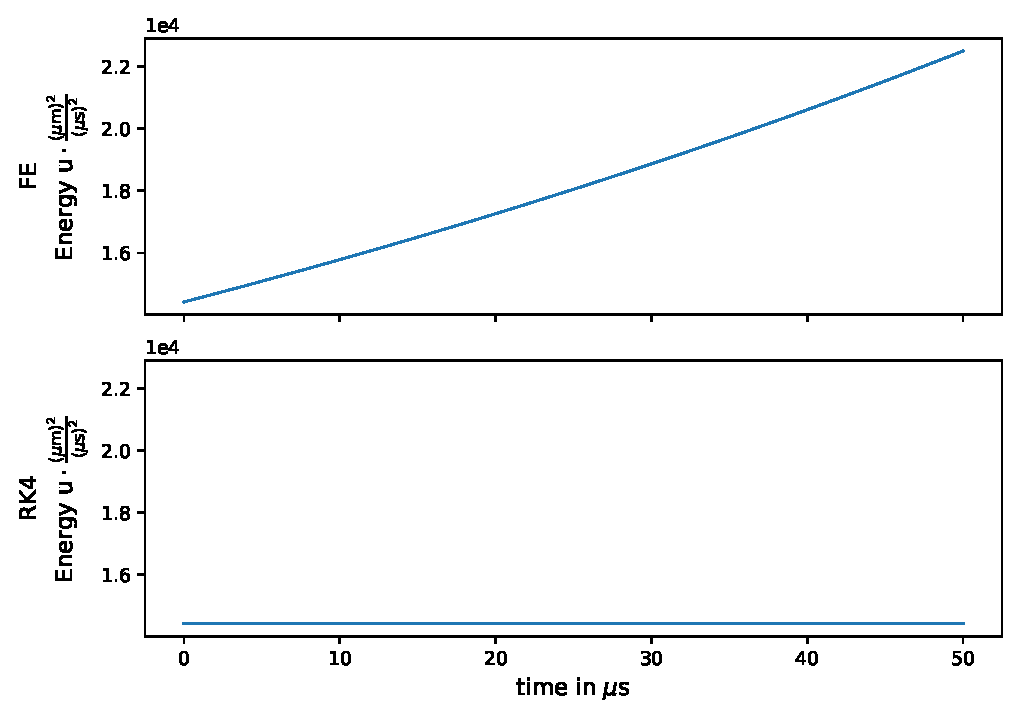
\includegraphics[width = 0.45 \textwidth]{Figures/RK4_vs_FE_total_energy.pdf}
    \caption{Total energy of the particle as a function of time. The upper plot shows the total energy in the FE simulation with 32000 time steps, the lower plot shows the total energy in the RK4 simulation with 32000 time steps.}
    \label{fig:energy}
\end{figure}

\Cref{fig:z-t-singleparticle} shows the particle's z-coordinate over the simulated time frame of $50 \mu s$ using both the FE (upper figure) and RK4 method (lower figure).
The vertical black lines show our expected upper and lower bounds for the particle's z position, as we expect this particle to move according to \cref{eq: zana}.
However, as discussed previously, neither FE nor RK4 is a symplectic method, and we do not expect them to accurately conserve energy.
When viewing the z-t-plot in the FE plot, this behaviour becomes obvious, as the simulated particle violates the theoretical maximum and minimum bounds of the z-coordinate. 
\footnote{This also becomes obvious when viewing an animation in the x-y-plane, where the circular motion in FE shows larger and larger circles. Such animations are saved under the  {\href{https://github.uio.no/johascha/CompPhys/tree/804b9bde4149b083d3da74c53a158c031194d2bb/Project_3/figures/Animations}{Animations folder}}.}

The failure of not conserving energy is also shown in \Cref{fig:energy}, where the total energy of the particle is displayed for both the FE and the RK4 method. 
We calculated this total energy as the sum of the kinetic energy of the particle and the potential energy given through the electric field and the charge of the ion.
The upper plot, which displays the energy of the particle in the FE, shows a near-constant energy drift. 
This causes the deviation from the analytical solution and would also be the cause for the simulated particle to not stay contained on a larger time scale, even though it is predicted to do so by the stability condition derived previously in section \cref{sec:penningtrap}.
In contrast, the more accurate RK4 method does not violate the bound in \Cref{fig:z-t-singleparticle}, as the method, in this case, is sufficiently more accurate to approach the real solution even after 50 $\mu s$. 
Furthermore, RK4 also does not show a significant energy drift in \Cref{fig:energy}, which is in line with what is seen in \Cref{fig:z-t-singleparticle}. 
Note that even though there is no significant energy drift observed in the simulation, RK4 can still cause drifts in the total energy. 
This was merely not observed here, because of the higher level of accuracy in comparison to FE and the high number of discretization points (32000).\\
In order to quantify the relative error of the calculations, our single particle simulation was compared to the analytical solution derived in \ref{sec:methods}.
To assess the accuracy, we defined the relative error as:
\begin{equation*}
    \epsilon_i = \frac{|\mathbf{r}_{i, \text{exact}} - \mathbf{r}_i|}{|\mathbf{r}_{i, \text{exact}}|}.
\end{equation*}

\begin{figure}[H]
    \centering
    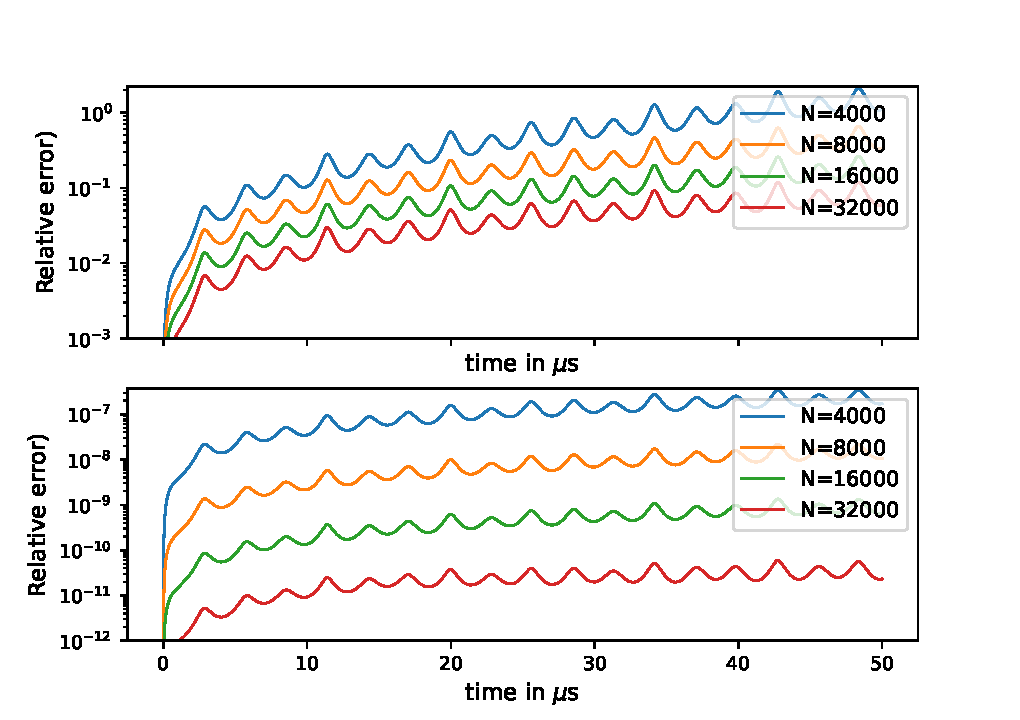
\includegraphics[width = 0.45 \textwidth]{Figures/RK4_vs_FE_rel_error-plot.pdf}
    \caption{Evolution of the relative error between the analytical and the numerical solution using FE (upper figure) and RK4 (lower figure). The differently coloured lines indicate different discretisation levels.}
    \label{fig:rel_error}
\end{figure}
The numerical superiority of RK4 can also be seen in \Cref{fig:rel_error}, where the relative error to the analytical solution is compared for different amounts of discretisation points.
To make the graphs more readable, the FE plot is cut off at a minimum relative error of $10^{-3}$, while the RK4 plot is cut off at a value of $10^{-12}$, with the y-axis being logarithmically scaled in both graphs.
As noted in \cref{sec:methods}, the FE has a global error of order $\mathcal{O}(dt)$, while the global error of RK4 is of order $\mathcal{O}(dt^4)$.

\begin{table}[ht]
    \centering
    \caption{Final relative errors for Forward Euler and RK4 methods.}
    \label{tab:error-comparison}
    \begin{tabular}{ccccc}
        \hline
        $\Delta t$ ($\mu\mathrm{s}$) &
        $\epsilon_{\mathrm{FE}}$ &
        $\epsilon_{\mathrm{RK4}}$ &
        $\epsilon_{\mathrm{FE}} / \Delta t$ &
        $\epsilon_{\mathrm{RK4}} / (\Delta t)^4$ \\
        \hline
        $1.25 \times 10^{-2}$ & $1.10$ & $1.70 \times 10^{-7}$ & $87.86$ & $6.98$ \\
        $6.25 \times 10^{-3}$ & $0.33$ & $1.07 \times 10^{-8}$ & $53.45$ & $6.98$ \\
        $3.13 \times 10^{-3}$ & $0.13$ & $6.58 \times 10^{-10}$ & $42.61$ & $6.90$ \\
        $1.56 \times 10^{-3}$ & $0.06$ & $2.31 \times 10^{-11}$ & $38.26$ & $3.88$ \\
        \hline
    \end{tabular}
\end{table}
\Cref{tab:error-comparison} shows the final relative errors for both FE and RK4 for all selected numbers of time steps.
The last two columns show the ratio between the final relative error and the step size to the power of the expected order of convergence for the two methods (1 for the FE method and 4 for the RK method).
These values are of interest, as the ratio between the final error and the suspected convergence order can approximately determine the order of convergence.
As the values of both of the last two columns stay approximately constant in magnitude, our expectations for the error of the FE method to be of order $\mathcal{O}(dt)$ and for the error of the RK4 method to be of order $\mathcal{O}(dt^4)$ are roughly confirmed.
It is of note that, especially for the FE method, the errors show slightly better convergence than expected.
However, as this convergence measure was only done at a single point, cancellation there may affect the observed order, leading to strongly suggestive rather than conclusive results.

\subsubsection*{Two Particle simulation}\label{sec:OnePart}

\Cref{fig:2-particle-nointer} shows the paths of two particles inside the Penning trap simulated using the RK4 algorithm with no interactions.
Particle 0 has the same initial conditions as the particle in the single particle simulation, while particle 1 is initialised at the position $\bold{r}=(25, 25, 0) \mu m$ with the velocity $\bold{v} = (0, 40, 5)\mu m/\mu s$.

\begin{figure}[ht]
    \centering
    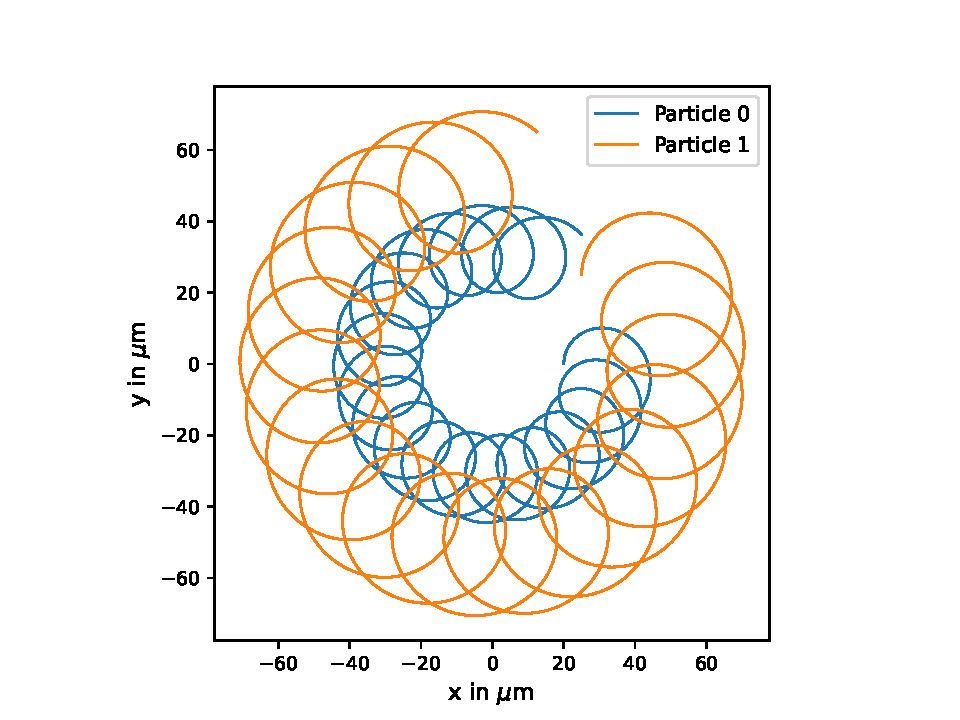
\includegraphics[width = 0.45 \textwidth]{Figures/RK_x_y_no_inter.pdf}
    \caption{The x-y-plane of two non-interacting particles inside the simulated Penning trap.}
    \label{fig:2-particle-nointer}
\end{figure}
As the underlying forces acting upon the particles have not changed in the case of no interaction, a similar picture as before arises.
Both particles perform two simultaneous orbital motions, comprised of a large orbit around the middle of the Penning trap, which is the magnetron drift, and a smaller, faster orbit, which is the cyclotron motion. 
This is in line with the analytical solution for single particles, which we found to be described by \cref{eq:Analyticalxy}, which features a superposition of two cylindrical motions.
In contrast, \Cref{fig:2-particle} shows the paths taken by two ions interacting through the Coulomb force, with the same initial conditions.
\begin{figure}[ht]
    \centering
    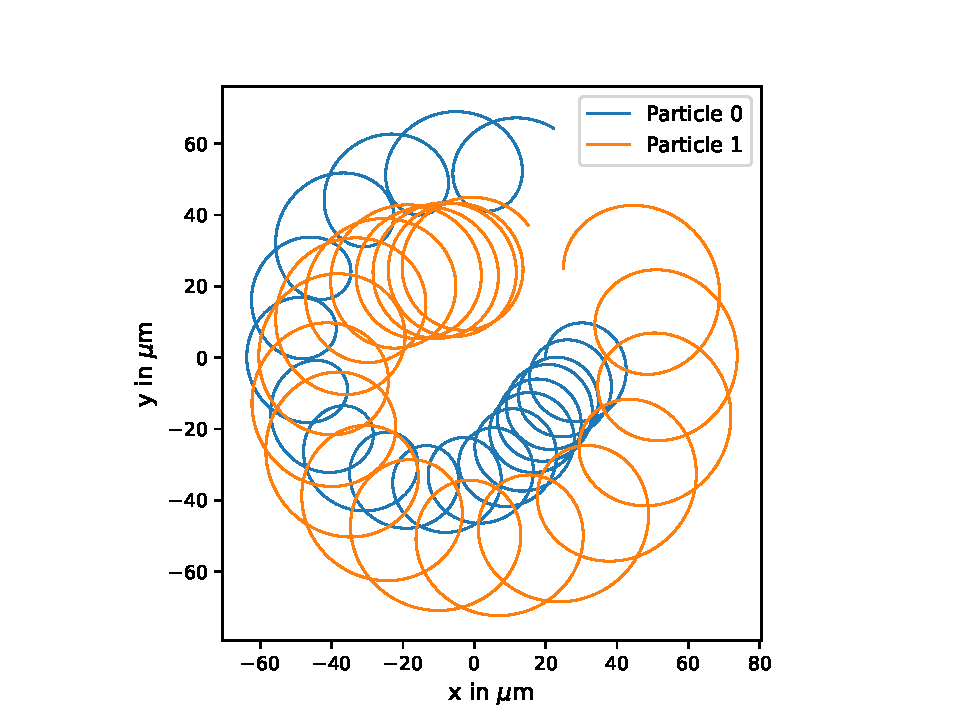
\includegraphics[width = 0.45 \textwidth]{Figures/RK_x_y.pdf}
    \caption{The x-y-plane of two particles interacting through the Coulomb force inside the simulated Penning trap.}
    \label{fig:2-particle}
\end{figure}

This creates significantly changed results for both of the particles, as the paths of the two particles now no longer orbit independently of each other.
Instead, the larger orbits of the two particles now overlap with each other, while the smaller, more frequent orbital motion shows varying speeds in comparison to the angular velocity of the larger orbital motion.
Both of these alterations can be explained through the introduction of the Coulomb force into the system.
While Particle 0 starts out further in the negative x direction than Particle 1, it will be pushed further in said direction, as long as Particle 1 has a larger x-coordinate.
A similar phenomenon can be seen in the y-direction. Here, Particle 1 has a larger y value at the start, however, due to the larger initial velocity and the initial position of the particle being further away from the origin, the y-value quickly shrinks below that of Particle 0.
During the time Particle 1 has a lower y value, it pushes Particle 0 into the positive y direction until it eventually reaches a higher y value towards the end of the simulation.
The transfer of energy through the Coulomb force couples the motion of the two particles, leading to a change in the angular velocity of both the cyclotron motion and the magnetron drift.
This therefore also explains the changes in the relative angular frequency between the two rotatory nodes.\\
The influence of the interactions through the Coulomb force can also be seen when viewing phase-space plots of the simulations.
\Cref{fig:phase-space-plots} shows both the x-$v_x$ and the z-$v_z$ phase space with and without interactions.

\begin{figure}[H]
    \centering
    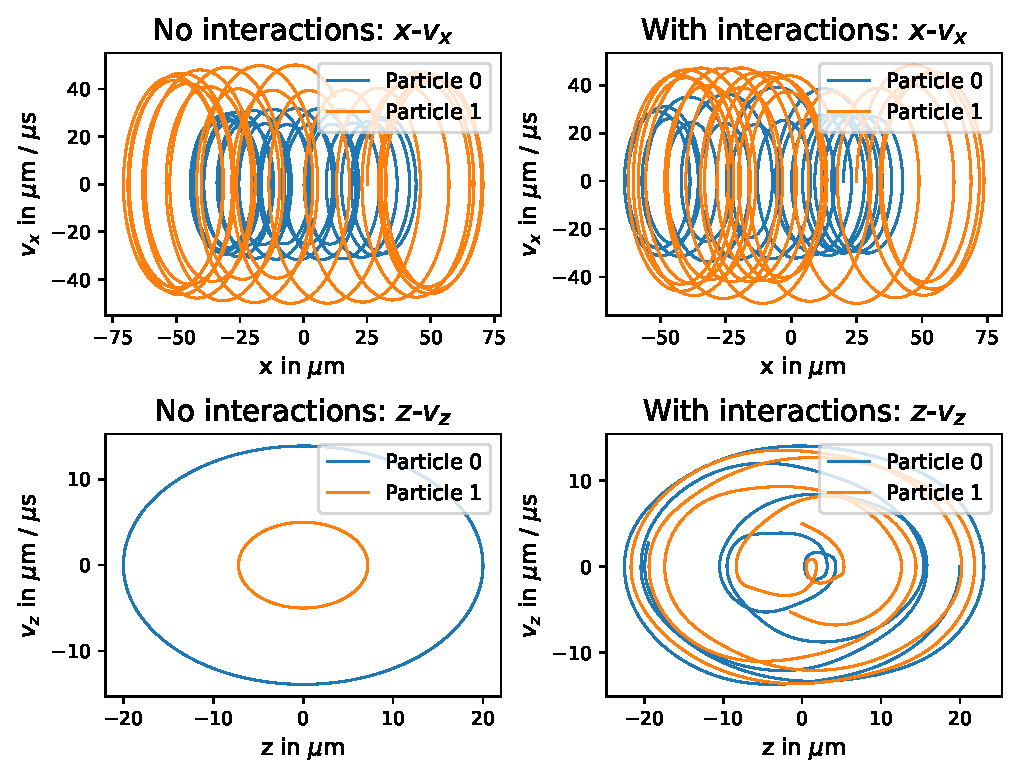
\includegraphics[width = 0.45 \textwidth]{Figures/RK4_two_particle_phase_space.pdf}
    \caption{The x-$v_x$ (upper row) and the z-$v_z$ (lower row) phase space in the RK4 simulation without (left column) and with interactions (right column).}
    \label{fig:phase-space-plots}
\end{figure}

While the z-$v_z$ phase space displays two stable oscillatory motions in the case of no interactions between the two particles, we can see clear coupling effects in the bottom right plot, which displays the z-$v_z$ phase space with interactions between the particles. 
This is in line with our expectation, as the repulsive Coulomb force transfers energy between the two particles, leading to continuous shifting in their phase space.
During this simulation of a 50 $\mu s$ time frame, both particles also remain bounded in the z-direction, as we previously had also seen in the x and y directions.


\subsubsection*{Perturbed Penning Traps}

The previously explored behaviour, although it brought great insight into how Penning traps work, was not entirely physical. That is because real-world experiments are not free of external perturbations, as was assumed. These perturbations can take various forms - for instance, the electromagnetic field can vary over time, potentially causing particles to escape the trap entirely. To investigate this possibility, we introduced a time-dependent term to the electric potential of our model:
\begin{equation}\label{eq:perturbation}
    V_0 \rightarrow V_0\left(1+f\cos(\omega_Vt)\right),
\end{equation}
where $f$ is a constant amplitude and $\omega_V$ is the angular frequency of the perturbation term.

Our subsequent analysis examined how the amplitude and angular frequency affect particle escape. The simulation setup consisted of 100 singly ionised Calcium-40 particles with randomised state vectors drawn from a normal distribution. The trap size and its magnetic field were kept as in previous tasks ($d=500$ $\mu\text{m}$, $B_0=1.00$ T), while the initial electric potential ($V_0=25.0$ mV) was perturbed according to eq. \ref{eq:perturbation}.

We then repeatedly simulated the evolution of the system for 500 $\mu$s with different values of $f$ and $\omega_V$, and counted how many particles were left inside the trap ($|\mathbf{r}|<d$). To get a coarse estimate of the resulting behaviour, we began with a broad sweep of angular frequencies ($\omega_V \in \left[0.2,2.5\right]$ MHz) with lower resolution to speed up computations ($d\omega = 0.02$ MHz). For each simulation, $40,000$ time steps were made, yielding $dt=0.0125$ $\mu$s. 

\begin{figure}
    \centering
    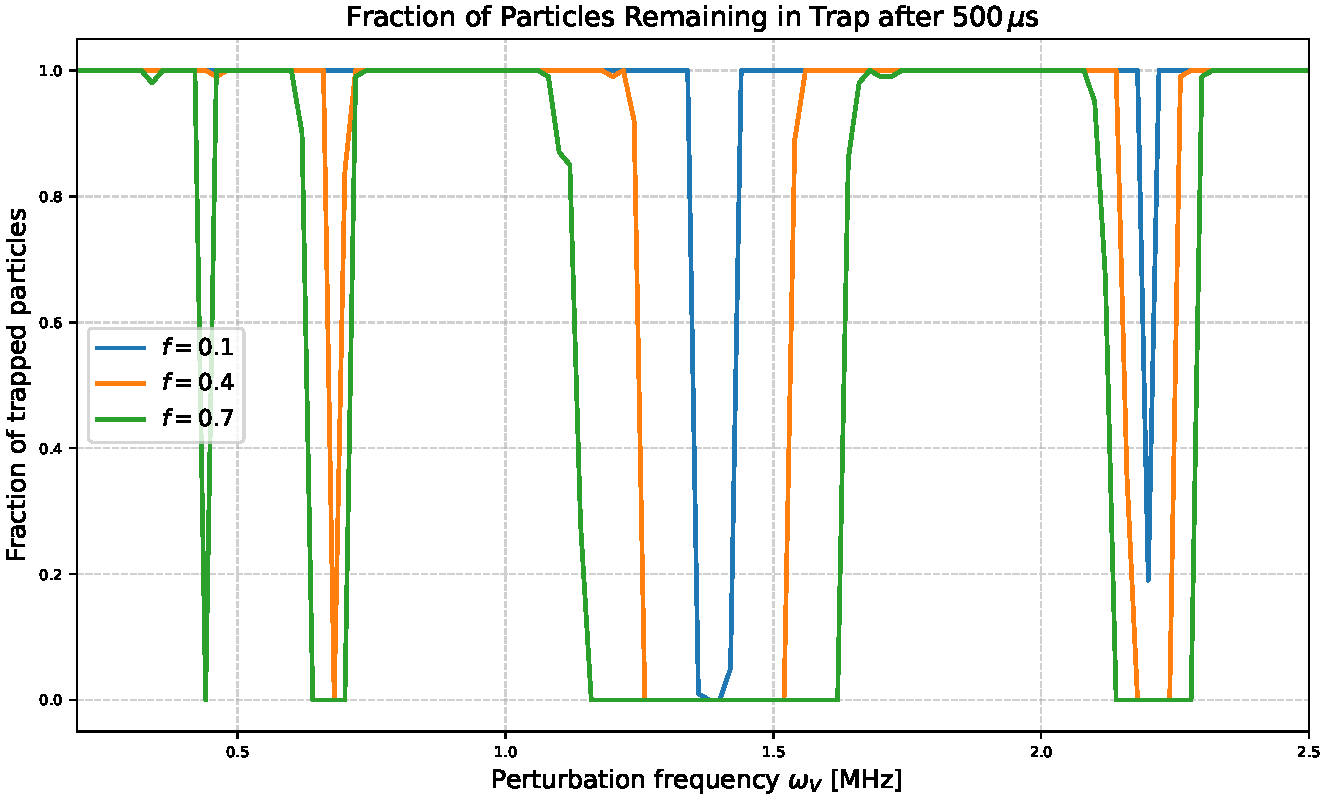
\includegraphics[width=1\linewidth]{Figures/coarse_resonance_sweep.pdf}
    \caption{Coarse sweep across a wide range of $\omega_V$}
    \label{fig:coarse_sweep}
\end{figure}

The results of the coarse analysis are plotted in fig. \ref{fig:coarse_sweep}. As can be observed, at certain perturbation frequencies, the number of remaining trapped particles after the simulation period drops sharply. This can be attributed to the phenomenon of resonance. When the period of particle oscillations within the trap aligns with the period of our harmonic perturbation, the minuscule `nudges' amplify constructively, pushing the particle away from the trap.

This effect is, somewhat predictably, strengthened for larger amplitudes, as indicated by the widening of resonance ranges at higher $f$. Bigger perturbation amplitudes exert greater influence on the particles, leading to more particles escaping at frequencies farther from the exact resonance.

Next, we performed a more detailed analysis around one of the discovered resonance frequencies ($\omega_V\approx1.39$ MHz). We narrowed the exploration window to $\omega_V \in \left[1.0,1.8\right]$ MHz and used a 10-times smaller $d\omega= 0.002$ MHz to increase the resolution. We also performed simulations for scenarios accounting and not accounting for inter-particle interactions (Coulomb). The time step was kept at $dt=0.0125$ $\mu$s due to the significantly increased computational workload in the inter-particle interaction version (the algorithm becomes $\mathcal{O}(n^2)$).

Figures \ref{fig:fine_sweep_inter} and \ref{fig:fine_sweep_nointer} present the results for scenarios with and without inter-particle interactions, respectively. The former is, due to its nature, inherently more chaotic. The random initial state vectors of the particles introduce noise to the picture, which has a more pronounced effect if the particles can interact. The lines in the no-interaction scenario graph are therefore noticeably smoother, but not perfectly smooth either (noise still has an effect). The previously observed behaviour for different perturbation amplitudes also holds in this finer regime -- larger $f$ leads to a broader region of particle escape around the resonant frequency.

\begin{figure}
    \centering
    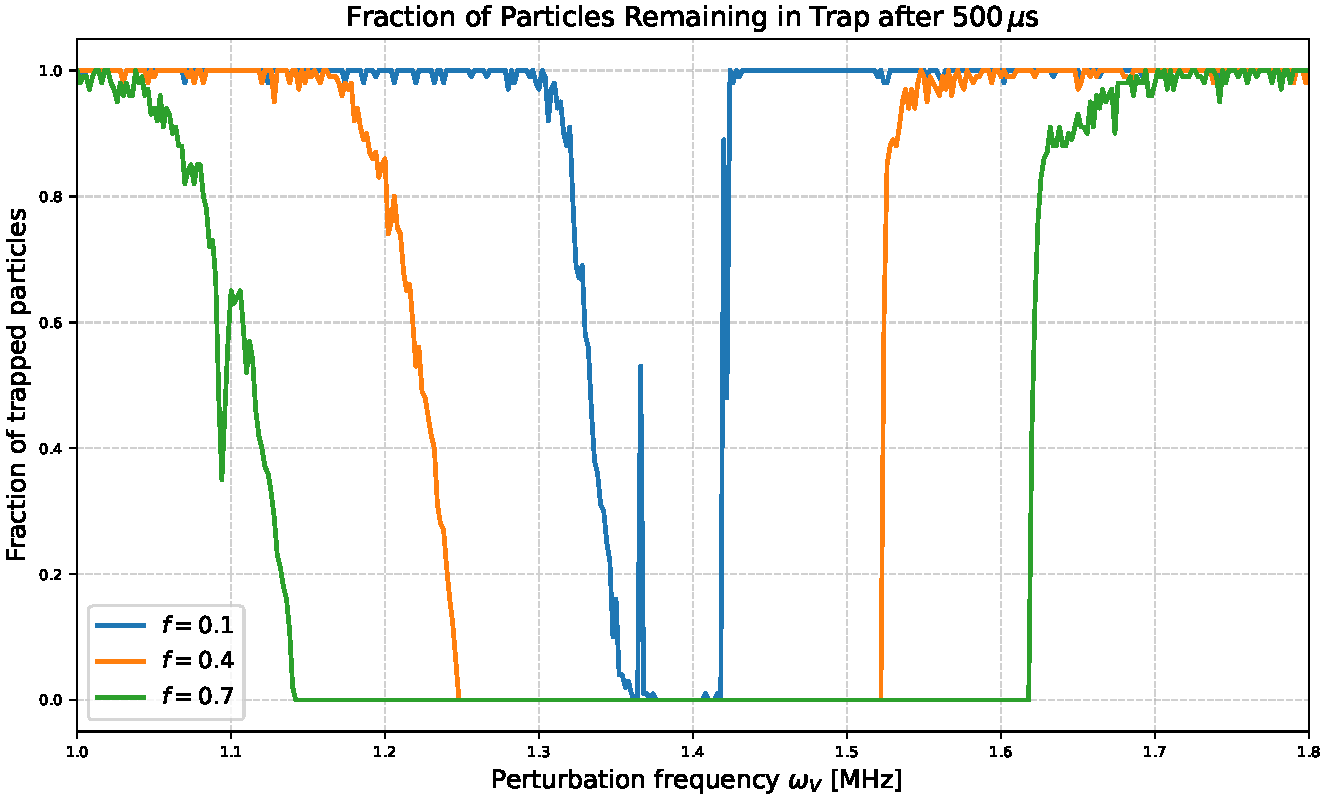
\includegraphics[width=1\linewidth]{Figures/fine_resonance_sweep_inter.pdf}
    \caption{Fine sweep across a narrow range of $\omega_V$, with inter-particle interactions}
    \label{fig:fine_sweep_inter}
\end{figure}

\begin{figure}
    \centering
    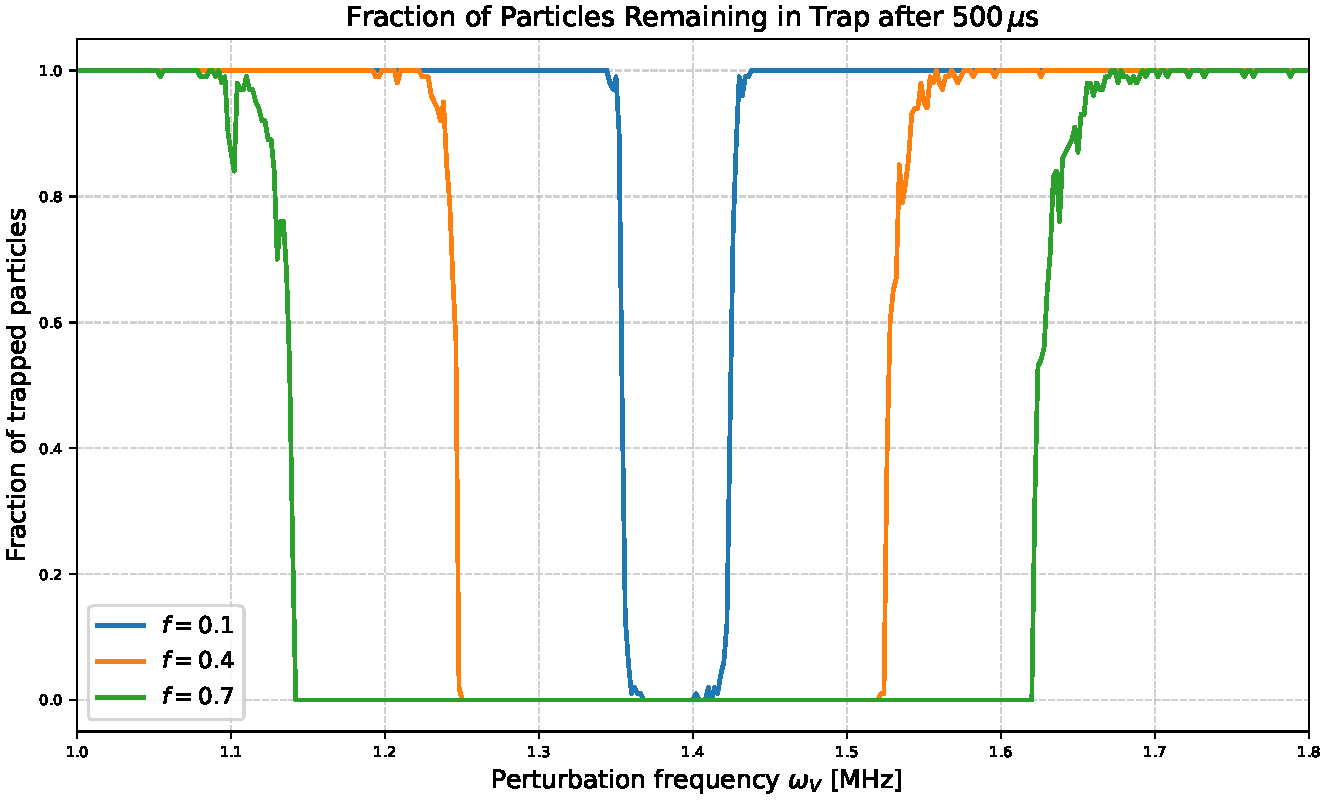
\includegraphics[width=1\linewidth]{Figures/fine_resonance_sweep_nointer.pdf}
    \caption{Fine sweep across a narrow range of $\omega_V$, without inter-particle interactions}
    \label{fig:fine_sweep_nointer}
\end{figure}

In the scenario that accounts for interactions, we also observe that the trap begins to lose particles farther from the resonant frequency. Interestingly, however, the slope is gradual, and the total loss of particles happens at approximately the same frequencies as in the no-interaction case.